\documentclass[a4paper,11pt]{amsart}
\usepackage{amssymb}
\usepackage{graphicx}

\parskip 1ex
\parindent 0 pt

\newcounter{temp}
\newcounter{prob_counter}
\newcounter{sprob_counter}

\newenvironment{problem}
{\begin{list}{{\bf \arabic{prob_counter}}}{
      \usecounter{prob_counter}
      \addtolength{\labelsep}{.6ex}
      \addtolength{\itemsep}{4.3ex}
      \setlength{\leftmargin}{1.4em}}
      \setcounter{prob_counter}{\value{temp}}
}
{\setcounter{temp}{\value{prob_counter}}  
  \end{list}
}

\newenvironment{subprob}
{
  \begin{list}{{\bf \alph{sprob_counter}}}{
      \usecounter{sprob_counter}
      \addtolength{\labelsep}{.6ex}
      \addtolength{\itemsep}{.5ex}
      \setlength{\leftmargin}{1.7em}}
}
{\end{list}}

\newenvironment{solution}{\textbf{Solution.}}{\qed}

\newcommand{\rubrik}[1]{\bigskip \begin{center}{\bf #1}\end{center} \medskip}

\newcommand{\NN}{\mathbb{N}}
\newcommand{\ZZ}{\mathbb{Z}}
\newcommand{\QQ}{\mathbb{Q}}
\newcommand{\RR}{\mathbb{R}}




\begin{document}

\pagestyle{empty}
\thispagestyle{empty}

{\small{\sc\noindent
        Tigran Tonoyan ({\tt tigran@ru.is}) and Tigran Tonoyan ({\tt tigran@ru.is})
}}

\rubrik{PROBLEM SET 2 (T-445-GRTH)}

You need to collect $\bf 65$ points to get a full score {\bf but} you cannot get more than {\bf X} points (in total) from a problem section with annotation {\bf max X}.

{\bf Please make sure to:}\\
1. Write your name/email(s) on your work (replace my name above).\\
2. Write your answers in \texttt{{\textbackslash}begin\{solution\} ... {\textbackslash}end\{solution\}} blocks given after each problem. Turn in a single \LaTeX-generated pdf.\\
3. Write clear and concise proofs: points may be deducted for vagueness.




\section{More on Trees ({\bf max 40}) }

\begin{problem}
\item (5 points)  
 Show that every tree $T$ has at least $\Delta(T)$ leaves, where $\Delta(T)$ denotes the maximum degree of $T$.
\end{problem}
\begin{solution}
\end{solution}

\begin{problem}
 \item (15 points) State necessary and sufficient conditions on an ordered $n$-tuple of positive integers
 $(d_1, \dots, d_n)$ with $d_1 \le d_2 \le \dots \le d_n$ in order that there be a tree $T$ on vertices $u_1, \dots, u_n$
 with $\text{deg}_T(u_i) = d_i$ for each $i \in \{1, \dots, n \}$. 
\end{problem}
\begin{solution}
\end{solution}

\begin{problem}
  \item (10 points) Let $\Delta \ge 3$, and let $d_{\Delta}(n)$ be the maximum number of nodes
 of degree $\Delta$ that a tree on $n$ vertices may have. Use induction to show that:
 \[
  d_{\Delta}(n) \le \left \lfloor \frac{n-2}{\Delta - 1} \right \rfloor.
 \]
\end{problem}
\begin{solution}
\end{solution}


\begin{problem}
\item \begin{subprob}
  \item (10 points) Show that if a tree $T$ has a longest path of even length, then the mid-vertex of one such longest path is the mid-vertex of every longest path in $T$. {\tiny Hint: First show that two such paths can't be vert.-disjoint.}
\item (5 points) Prove that the common vertex is a center of $T$.
\end{subprob}
\end{problem}
\begin{solution}
\end{solution}


\begin{problem}
 \item (5 points) A full ternary tree is an ordered rooted tree where each vertex, except the leaves, has 
 exactly $3$ children. Hence, all of the internal vertices have degree four, except the root which has degree 
 $3$. Prove the \textit{Full Ternary Tree Theorem} which states that a regular ternary tree has $n = 3k+1$ vertices,
 $k$ of them internal and $2k+1$ of them leaves.
\end{problem}
\begin{solution}
\end{solution}



\section{Spanning Trees ({\bf max 15})}


\begin{problem}
 \item (7 points) Describe a procedure for finding a spanning tree in a graph. Prove that it indeed finds a spanning tree in every connected graph. Apply it to the graph from the following exercise.
\end{problem}
\begin{solution}
\end{solution}


\begin{problem}
 \item (10 points) How many different spanning trees does the following graph contain?
\begin{center} 
 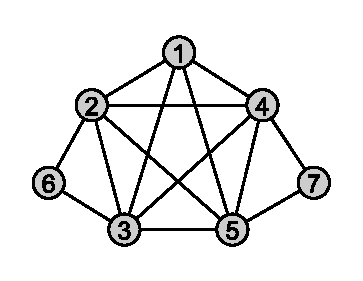
\includegraphics[height=4cm]{st-count.pdf}
\end{center}
\end{problem}
\begin{solution}
\end{solution}



\section{Eulerian Graphs ({\bf max 25})}

\begin{problem}
\item
 Consider the $3 \times 3$ chessboard, and let $Q$ denote the $9$ squares of the board. Let 
 $H_{3,3} = (Q, E)$ denote the simple graph on vertex set $Q$ so that $(q_1, q_2) \in E$ if and 
 only if a rook at square $q_1$ can reach $q_2$ in a single move (a rook can move 
 horizontally and vertically  arbitrary distance).
\begin{subprob}
 \item (5 points) Run \textit{Fleury's algorithm} for computing an Eulerian circuit on $H_{3,3}$. The algorithm on a simple graph $G=(V,E)$ is as follows: 
 \begin{quote}
 Pick a vertex $v_1$ arbitrarily. Having picked $v_1, \dots, v_k$,  set 
 $G_k = G \, - \, \{e_{1,2}, e_{2,3}, \dots, e_{{k-2},{k-1}}, e_{{k-1},k} \}$, where $e_{i,j}$ denotes
 an edge connecting $v_i$ to $v_j$.
 If there is a non-bridge (in $G_k$) edge connecting $v_k$ to a vertex $u$ then let 
 $v_{k+1} = u$. Otherwise, let $v_{k+1}$ be any neighbor of $v_k$ in $G_k$. If the degree of $v_k$ in
 $G_k$ is $0$ then terminate. Repeat. 
 \end{quote}
 
\item  (5 points) Consider the general $n \times m$ chessboard, for $n,m \ge 1$, and similarly the graph $H_{n,m}$ so that two vertices (squares) are adjacent if and only if a rook can get from one to the other in one move. For which values $n,m$ does the graph $H_{m,n}$ contain a Euler circuit?
 \item (10 points) Prove that Fleury's algorithm always finds an Eulerian circuit if there is one. 
\end{subprob}
\end{problem}
\begin{solution}
\end{solution}


\begin{problem}
\item (10 points) For an integer $k$, let $G$ be a connected graph that contains $2k$ vertices of odd degree. Show that there exist $k$ edge-disjoint subgraphs $G_1, \dots, G_k$ such that
 \begin{itemize}
  \item $E(G) = E(G_1) \cup E(G_2) \cup \dots \cup E(G_k)$,
  \item each $G_i$ has an Eulerian trail.
 \end{itemize}
 
\tiny{Hint: Add $k$ edges to $G$ so that it becomes Eulerian.}
\end{problem}
\begin{solution}
\end{solution}


\begin{problem}
 \item (5 points) Prove that a balanced weakly connected graph is strongly connected.
\end{problem}
\begin{solution}
\end{solution}



\section{Hamiltonian Graphs ({\bf max 20})}



\begin{problem}
 \item (10 points) Let $m$ and $n$ be positive integers. Consider the \textit{grid graph} $G_{m,n} = (V, E)$ with vertex set $V = \{1, \dots, m\} \times \{1, \dots, n\}$, where vertices $u = (x, y) \in V$ and $v = (x', y') \in V$ are adjacent if and only if $|x - x'| + |y - y'| = 1$. Find necessary and sufficient conditions that $m$ and $n$ must satisfy in order for the graph $G_{m,n}$ to be Hamiltonian.
\end{problem}
\begin{solution}
\end{solution}


\begin{problem}
 \item (10 points) Prove that the following graph is not Hamiltonian.
 \begin{center}
  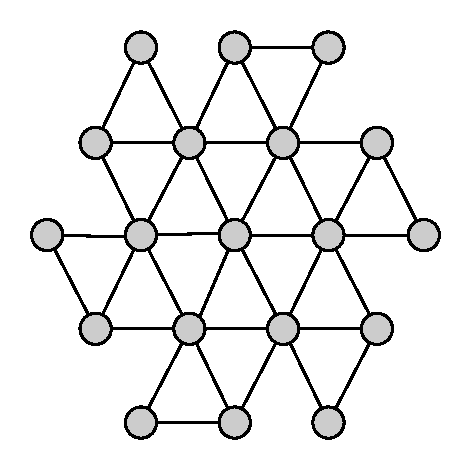
\includegraphics[height=5cm]{hamiltonian.pdf}
 \end{center}
\end{problem}
\begin{solution}
\end{solution}






\section{Connectivity ({\bf max 30})}


\begin{problem}
 \item (5 points) Show that a vertex $u$ in a graph $G$ is a cut-vertex if, and only if, there are vertices $v, w \in V(G) \setminus \{u\}$ such that every path between $v$ and $w$ contains the vertex $u$.
\end{problem}
\begin{solution}
\end{solution}


\begin{problem}
 \item (10 points) Show that if $G$ is a graph on $n$ vertices and $m$ edges, we have:
 \[
  \kappa(G) \le \kappa'(G) \le \left\lfloor \frac{2m}{n} \right\rfloor .
 \]
\end{problem}
\begin{solution}
\end{solution}


\begin{problem}
 \item (10 points) Let $G$ be a connected graph. Show that if $C \subseteq E(G)$ has an even number of edges in common with every edge cut of $G$, then $C$ is an edge-disjoint union of cycles.
\end{problem}
\begin{solution}
\end{solution}


\begin{problem}
 \item (5 points) For a tree $T$ on $n$ vertices and with maximum degree $\Delta$,
 what is the minimum number of vertices in its block-cutpoint graph $BC(T)$? 
\end{problem}
\begin{solution}
\end{solution}




\end{document}

